\chapter{Analisis Persoalan dan Rancangan Solusi}

Tujuan utama penulisan bab ini adalah untuk menguraikan rencana penyelesaian masalah pencarian kondisi ketika \textit{erasure coding} memiliki \textit{response time} yang lebih cepat dibandingkan replikasi. Bagian ini memaparkan proses analisis masalah hingga menjadi solusi.


\section{Analisis}

\section{Analisis Permasalahan}
\label{sec:analisis-permasalahan}

% Berdasarkan latar belakang yang telah diuraikan pada \ref{sec:latar-belakang}, penggunaan \textit{erasure coding} pada sebuah sistem dapat mengurangi kebutuhan penyimpanan data dengan tetap menjaga integritas dan ketahanan data. Walaupun membutuhkan sumber daya komputasi dalam penerapannya, pengurangan ukuran data keseluruhan yang diperlukan menyebabkan juga turunnya ukuran data yang perlu dikirim ke \textit{node} lainnya.Hal ini menyebabkan mungkinnya terdapat suatu kondisi ketika {response time} yang diperlukan untuk melakukan operasi pada \textit{erasure coding} lebih rendah jika dibandingkan dengan melakukan operasi yang sama pada sistem yang menggunakan \textit{replikasi} untuk mencapai ketahanan tersebut.

Berdasarkan latar belakang dan studi literatur yang telah ditentukan, \textit{erasure coding} memiliki potensi untuk menghasilkan \textit{response time} yang lebih rendah dibandingkan dengan sistem berbasis \textit{replikasi} karena walaupun membutuhkan komputasi, ukuran data yang dikirimkan untuk ketahanan lebih rendah dibandingkan replikasi. Riset ini akan menganalisis faktor-faktor untuk mencapai kondisi tersebut. Faktor yang dianalisis antara lain ukuran data yang besar dan jaringan yang lambat. Dengan demikian, diperlukan sistem yang dapat mensimulasikan operasi pada sistem \textit{erasure coding} dan replikasi sekaligus memvariasikan faktor-faktor tersebut dalam operasinya tanpa memengaruhi kinerja sistem di sisi lain.

Dari permasalahan tersebut, dirumuskan kebutuhan sebuah perangkat lunak antara lain
\begin{enumerate}

    \item Sistem harus dapat mensimulasikan kondisi \textit{database} terdistribusi yang menggunakan replikasi ataupun \textit{erasure coding}.
    \item Sistem harus dapat menyimpan data secara \textit{persistent}.
    \item Sistem harus dapat memvariasikan ukuran data dan kecepatan jaringan.
    \item Sistem harus dapat menjalankan eksperimen berulang kali untuk mendapatkan data dari eksperimen.

\end{enumerate}

Penjelasan lebih detail mengenai kebutuhan sistem terdapat pada lampiran \ref{sec:rancangan-struktural}.

\subsection{Alternatif Solusi}
\label{sec:alternatif-solusi}

Berdasarkan permasalahan pada bagian \ref{sec:analisis-permasalahan}, terdapat berbagai macam alternatif solusi untuk menyelesaikan permasalahan tersebut. Pada penelitian ini, solusi yang dipilih adalah dengan membuat sistem yang mengkombinasikan Memcached sebagai \textit{in-memory key value store} dengan RocksDB sebagai \textit{persistent storage} dengan Reed-Solomon sebagai algoritma \textit{erasure coding}.

\subsubsection{Perbandingan Pengembangan Sistem}

Terdapat beberapa solusi yang dipertimbangkan dalam pembangunan sistem, yaitu membangun sistem dengan 

\begin{enumerate}
  \item Mengembangkan sistem secara modular dengan in-memory key-value store dan persistent storage terpisah
  
  Pendekatan ini mengkombinasikan antara sistem \textit{in-memory key-value store} dengan menggunakan \textit{database} terpisah sebagai tempat penyimpanan data \textit{persistence}. Replikasi dan \textit{erasure coding} dapat dilakukan pada data persisten yang disimpan pada \textit{database} tersebut. Kelebihan dari pendekatan ini adalah kemudahan dari implementasi dibandingkan pengembangan sendiri ataupun modifikasi \textit{database} yang sudah lebih kompleks. Namun, kekurangannya adalah \textit{overhead} penggunaan memori dari menjalankan \textit{in-memory key-value store} dan \textit{database} terpisah. Dari ketiga alternatif solusi, kemudahan implementasi dan kekurangan yang dapat ditoleransi menjadikan alternatif ini solusi yang dipilih dalam penelitian ini.


  \item Mengembangkan sistem mock database
  
  Pendekatan ini membangun semua fitur-fitur yang dibutuhkan secara mandiri. Kelebihan dari pendekatan ini kebebasan yang tinggi sehingga sistem dapat disesuaikan untuk eksperimen. Namun, pendekatan ini sulit mencerminkan kondisi nyata. Selain itu, kinerja sistem yang dikembangkan juga bergantung erat pada waktu serta kemampuan pengembangan peneliti.

  \item Mengembangkan sistem yang sudah memiliki fitur in memory database dan persistent storage
  
  Pengembangan ini membangun mengganti fitur yang dibutuhkan untuk penelitian di atas \textit{database} lebih kompleks dari Memcached. Pendekatan ini memiliki kelebihan kedekatan kondisi eksperimen dengan dunia nyata. Namun, pendekatan ini sulit dilakukan karena membutuhkan waktu yang lama untuk memahami dan mengubah \textit{source-code database} yang kompleks.
\end{enumerate}

\subsubsection{Perbandingan Kakas}
Setelah menentukan solusi pengembangan sistem secara modular, terdapat beberapa kakas yang dapat dipilih untuk solusi tersebut. Disebabkan pemilihan solusi modular, kakas yang dipertimbangkan untuk digunakan meliputi kakas \textit{in-memory key-value store} dan kakas untuk \textit{persistent database}.

\begin{enumerate}
    \item In-memory key-value store
    
    Memcached dipilih sebagai \textit{in-memory key-value store}. Selain Memcached, kakas yang dipertimbangkan untuk digunakan sebagai \textit{in-memory key-value store} adalah seperti yang ada pada tabel \ref{tab:tools-kv} \parencite{redis_docs} \parencite{dragonflydb_docs} \parencite{memcached_docs}.

    \begin{table}[h]
        \centering
        \caption{Perbandingan kakas in-memory key-value store}
        \resizebox{\textwidth}{!}{
            \begin{tabular}{|l|p{5cm}|p{5cm}|p{3cm}|}
                \hline
                \rowcolor{black!10} Kakas & Kelebihan & Kekurangan & Notes \\ \hline
                Redis & +Support struktur data kompleks \newline +Support transaksi kompleks & -Single Threaded \newline -Kompleks & Ada support untuk replikasi \\ \hline
                DragonflyDB & +Multithreaded \newline +Support struktur data kompleks \newline +Support transaksi kompleks & -Lebih kompleks dari Memcached, lebih simpel dari Redis \newline -Relatif baru, komunitas terbatas dibanding kedua alternatif & Rilis 2023, Ada support untuk replikasi\\ \hline
                Memcached & +Simpel \newline +Multithreaded & -Struktur data terbatas \newline -Transaksi terbatas & Sangat minimalis \\ \hline
            \end{tabular}
        }
        \label{tab:tools-kv}
    \end{table}

    Dari kakas-kakas tersebut, dipilih Memcached sebagai kakas untuk eksperimen ini. Alasan utama pemilihan Memcached adalah sifatnya yang paling simpel, kinerja \textit{multithreaded}-nya, serta tidak dibutuhkannya fitur-fitur yang dimiliki Redis dan Dragonfly.
    
    \item Persistent database
    
    RocksDB dipilih sebagai \textit{persistent storage} karena berfokus pada kinerja \textit{write} yang tinggi. Penggunaan RocksDB juga dilakukan seperti \textit{library} sehingga memudahkan pengembangan sistem yang modular. Selain RocksDB, kakas yang dipertimbangkan untuk digunakan sebagai \textit{persistent database} adalah seperti yang ada pada tabel \ref{tab:tools-db} \parencite{cassandra_docs} \parencite{scylladb_docs} \parencite{rocksdb_docs} \parencite{leveldb_docs} \parencite{mongodb_docs}.

    \begin{table}[h]
        \centering
        \caption{Perbandingan kakas persistent database}
        \resizebox{\textwidth}{!}{
            \begin{tabular}{|l|p{5cm}|p{5cm}|p{3cm}|}
                \hline
                \rowcolor{black!10} Kakas & Kelebihan & Kekurangan & Notes \\ \hline
                Cassandra & +Horizontal Scalability baik \newline +Sudah ada referensi implementasi erasure coding pada paper lain & -Eventual Consistency \newline -Latensi tinggi untuk operasi write \newline -Sangat Kompleks & Utamanya Wide-Column Store\\ \hline
                ScyllaDB & +Lebih efisien dan performant dibandingkan Cassandra \newline +Memiliki pilihan strong consistency & -Lebih kompleks dibandingkan Cassandra \newline -Ekosistem terbatas & Mirip dan kompatibel dengan Cassandra. \\ \hline
                RocksDB & +Kinerja tinggi untuk operasi write \newline +Recovery menggunakan write ahead log & -Single Node \newline -Keterbatasan pada concurrent writes & Pengembangan LevelDB\\ \hline
                LevelDB & +Simpel \newline +Penggunaan memori kecil \newline +Kinerja tinggi untuk operasi write & -Fitur terbatas seperti compression dan data terbatas pada string \newline -Operasi write skala besar masih lebih lambat dibandingkan RocksDB \newline -Keterbatasan pada concurrent writes & Dasar dari RocksDB\\ \hline
                MongoDB & +Support query kompleks \newline +Penggunaan fleksibel & -Operasi kurang optimal \newline -Konsumsi memori besar \newline -Storage overhead besar & Utamanya Dokumen database\\ \hline
            \end{tabular}
        }
        \label{tab:tools-db}
    \end{table}

    Dari kakas-kakas tersebut, dipilih RocksDB sebagai kakas untuk eksperimen ini. Selain RocksDB, LevelDB juga merupakan kandidat yang kuat untuk eksperimen ini karena sifatnya yang simpel. Namun, pada akhirnya, RocksDB dipilih karena pengembangannya yang masih aktif, kinerja \textit{write} yang lebih tinggi, serta fitur-fitur tambahan seperti \textit{compression} dan penyimpanan data dalam \textit{byte}.

\end{enumerate}

\subsubsection{Perbandingan Algoritma Erasure Coding}
Terdapat beberapa algoritma yang dipertimbangkan untuk implementasi \textit{erasure coding} selain Reed-Solomon \parencite{manasse2009reed}. Algoritma tersebut antara lain adalah kode LDPC (\textit{Low-Density Parity-Check}) \parencite{gallagher1962ldpc}, kode BCH (\textit{Bose-Chaudhuri-Hocquenghem}) \parencite{bose1960bch}, algoritma berbasis XOR (Terdapat berbagai macam sumber dan implementasi untuk algoritma XOR), kode Fountain \parencite{asteris2014fountain}, dan \textit{Regenerating Codes} \parencite{rashmi2012regenerating}. Berikut perbandingan masing-masing algoritma 

\begin{table}[ht]
    \centering
    \caption{Perbandingan algoritma erasure coding}
    \resizebox{\textwidth}{!}{
        \begin{tabular}{|l|l|p{3cm}|p{2.2cm}|p{3cm}|p{3cm}|}
            \hline
            \rowcolor{black!10} Algoritma & Basis & Komputasi & Distance & Kelebihan & Kekurangan \\ \hline
            Reed-Solomon & Block level & Polynomial Interpolation & Optimal & Efisiensi penyimpanan tinggi & Komputasi kompleks \\ \hline
            LDPC Codes & Bit level & Sparse Matrix operations & Hampir \newline Optimal & Kecepatan \textit{encoding/decoding} tinggi untuk \textit{data streaming} & Membutuhkan \textit{overhead} untuk operasi \textit{block}  \\ \hline
            BCH Codes & Block level & Syndrome decoding & Optimal & Efisien untuk \textit{burst errors} & Kompleksitas meningkat dengan ukuran data \\ \hline
            XOR-based & Bit level & XOR operations & Optimal & Komputasi sangat sederhana & Kemampuan pemulihan data terbatas\\ \hline
            Fountain Codes & Symbol level & Linear encoding/decoding & Probabilistik & Menghasilkan \textit{encoding} tidak terbatas & Bersifat probabilistik \\ \hline
            Regenerating Codes & Block level & Linear encoding/decoding & Optimal & \textit{Bandwidth} lebih rendah dibanding Reed-Solomon untuk repair & Kompleksitas koordinasi dan overhead penyimpanan antar node tinggi  \\ \hline
        \end{tabular}
    }
    \label{tab:ec-algorithm}
\end{table}

Distance adalah nilai \textit{overhead} memori algoritma tersebut dalam mengatasi kegagalan \textit{node}. Nilai distance optimal adalah $k + m = n$ dimana $k$ adalah jumlah \textit{data block}, $m$ adalah jumlah \textit{parity block}, dan $n$ adalah jumlah total \textit{block} yang dibutuhkan. Simbol yang sama digunakan untuk redundansi. Penjelasan implementasi dapat dilihat pada referensi masing-masing algoritma.


\subsection{Analisis Kebutuhan Sistem}
\label{sec:analisis-kebutuhan-sistem}

Berdasarkan bagian \ref{sec:analisis-solusi}, ::TODO: fill::.


\section{Rancangan}

\subsection{Arsitektur Sistem}
\label{subsection:system-architecture}

\begin{figure}[ht]
    \centering
    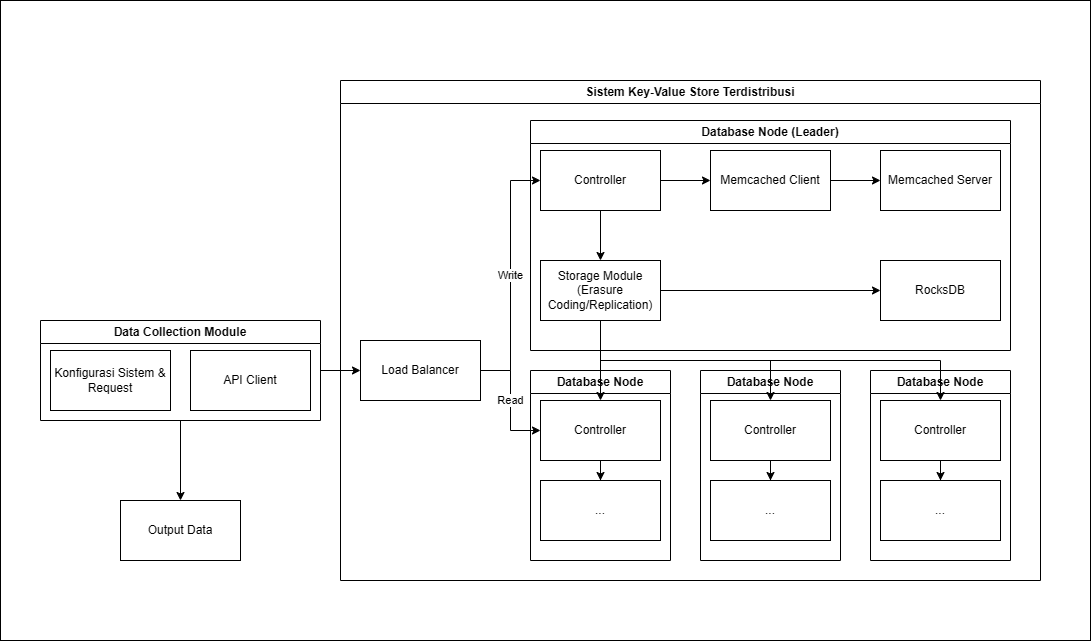
\includegraphics[width=0.95\textwidth]{resources/chapter-3/general-architecture.png}
    \caption{Gambaran Arsitektur Sistem Eksperimen}
    \label{fig:general-architecture}
\end{figure}

Arsitektur dari sistem mengasumsikan kebutuhan untuk konsistensi yang tinggi. Untuk mencapai konsistensi tersebut, operasi \textit{write} dilakukan secara \textit{synchronous} dengan distribusi replikasi dan \textit{erasure coding} dianggap selesai ketika nilai ketahanan yang diinginkan sudah tercapai.

Karena sistem bersifat terdistribusi, maka diperlukan sebuah algoritma konsensus untuk mengelola konsistensi antar \textit{Node}. Algoritma konsensus yang digunakan algoritma konsensus \textit{paxos} yang disesuaikan dengan kebutuhan. Salah satu penyesuaian yang dilakukan adalah mengadopsi pola \textit{leader-follower} untuk memudahkan sinkronisasi data dan mempercepat transaksi. Dengan adanya leader, fase 1 dari algoritma \textit{paxos} dapat dihilangkan dengan membuat proposal dari leader selalu memiliki nilai paling tinggi. Detail implementasi \textit{paxos} akan dijelaskan di bagian \ref{subsection:detail-komponen}. Diagram gambaran arsitektur sistem dapat dilihat pada gambar \ref{fig:general-architecture}.

Operasi \textit{write} akan secara ekslusif disalurkan pada \textit{leader}. Kemudian untuk ketahanan, data akan didistribusikan pada \textit{follower} sesuai dengan konfigurasi \textit{node}. Sementara itu, operasi \textit{read} dapat dilakukan pada \textit{Node} manapun. Pada sistem \textit{erasure coding}, jika pada \textit{node} tersebut tidak terdapat nilai data yang dicari, maka \textit{Node} akan melakukan \textit{request} ke semua node lainnya untuk melakukan rekonstruksi data.

